\chapter{Computational Experiments}
\label{chap:experiments}


This chapter describes the main computational experiments made in this work. First, general computational aspects are introduced; then different scenarios for different schools are described; and finally results are presented and evaluated.


%%%%%%%%%%%%%%%%%%%%%%%%%%%%%%%%%%%%%%%%%%%%%%%%%%%%%%%%%%%%%%%%%%%%%%%%%%%%%%%%%%
\section{General}

The implementation of the solver was done in C++, compiled with MS Visual Studio 2010 environment, using Microsoft Windows 7, 64 bits.

All the linear integer programs were solved using the generic MIP-Solver Gurobi 6.0. 

Computational experiments were executed on 3.40GHz Intel Core i7 computer with 32 GB of RAM. Considering all scenarios, the maximum observed amount of RAM being used by the solver during execution was around 7 GB.


%%%%%%%%%%%%%%%%%%%%%%%%%%%%%%%%%%%%%%%%%%%%%%%%%%%%%%%%%%%%%%%%%%%%%%%%%%%%%%%%%%
\section{Scenarios}

Several computational experiments have been performed for real scenarios of Brazilian schools. Those considered the most significant are following detailed.

General features of scenarios:
\begin{table}[ht]
\caption{Scenarios} 							% title of Table
\centering
\begin{tabular}{c c c c c} 							% centered columns
\hline\hline 											% inserts double horizontal lines
Scenario & Classes & Credits demanded & Teaching staff available credits & Blocks \\ [0.5ex] 						% heading
\hline 														% inserts single horizontal line
A & 178 & 5800 & 9154 & 14 \\
B1 & 295 & 9490 & 15249 & 15 \\
B2 & 295 & 9490 & 15243 & 15 \\
C & & & & \\
D & & & & \\
E & & & & \\ [1ex] 							% [1ex] adds vertical space
\hline
\end{tabular}
\label{table:scenarios} 					% is used to refer this table in the text
\end{table}



Detailed features of scenarios:
\begin{table}[ht]
\caption{Scenarios} 							% title of Table
\centering
\begin{tabular}{c | c c c c c c} 	% centered columns
\hline\hline 											% inserts double horizontal lines
\multirow{2}{*}{Features} &
	\multicolumn{6}{c}{Scenarios} \\
																				& A & B1 & B2 & C & D & E \\ [0.5ex] 						% heading
\hline 														% inserts single horizontal line
Classes 																& 178	& 295	 & 295& & \\
Demanded credits 												& 5800	& 9490 & 9490& & \\
Average of demanded credits per class 	& 32.5843	& 32.1695	 & 32.1695& & \\
\hline
Professors 															& 	& 	 & & & \\
Professors available credits 						& 9154	& 15249	 & 15243& & \\
1st-priority professors available credits & 	& 	 & & & \\
2nd-priority professors available credits	& 	& 	 & & & \\
\hline
Blocks 																	& 14	& 15	 & 15& & \\
Min/Max classes per block 							& 2/29	& 9/28 & 9/28& & \\
Average of classes per block 						& 	& 	 & & & \\

 [1ex] 							% [1ex] adds vertical space
\hline
\end{tabular}
\label{table:scenarios} 					% is used to refer this table in the text
\end{table}




\begin{enumerate}
%---------------
\item A: Pensi - sem noite - com amarracao de disponib por unidade

\begin{figure}[H]
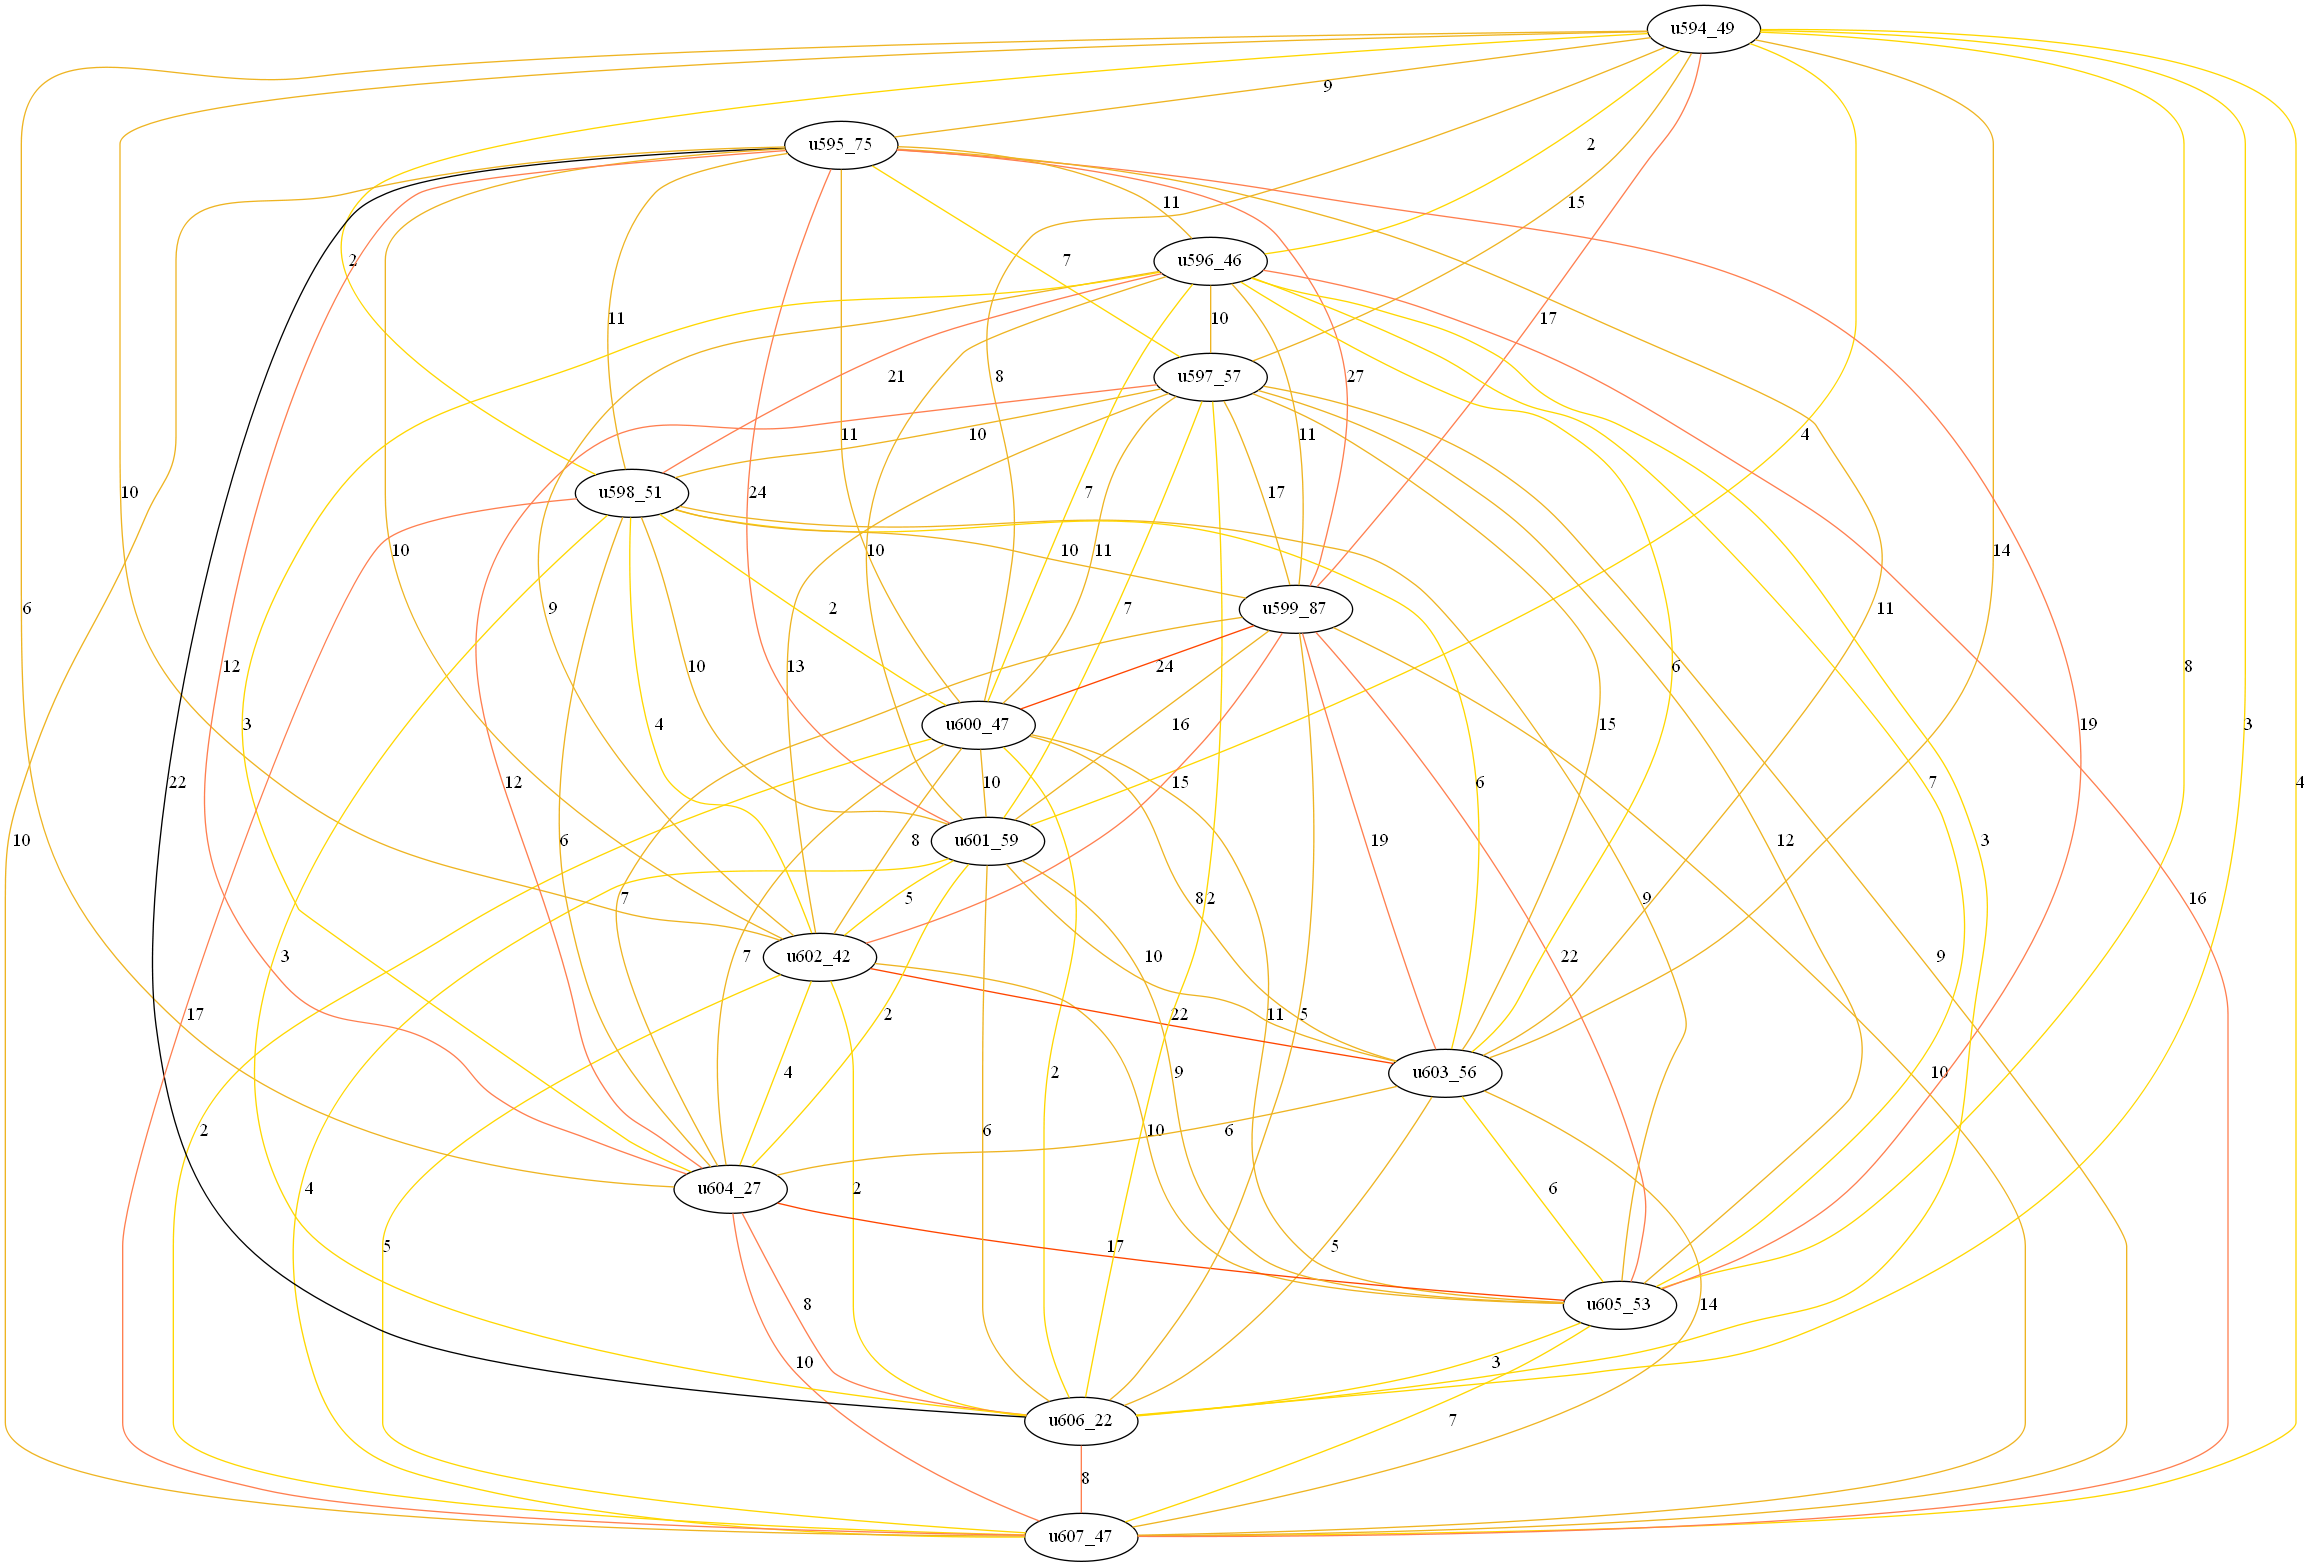
\includegraphics[scale=1.0]{"Computational Experiments/Inputs/inputPensiSemNoitePriorProfs_201501291331550_/parUnidProfsComuns-PensiSemNoitePriorProfs_201501291331550.png"}
\centering
\caption{Sharing of professors between blocks (school units) of scenario A}
\end{figure}

%---------------
\item B1: Elite - sem amarracao de disponib por unidade

\begin{figure}[H]
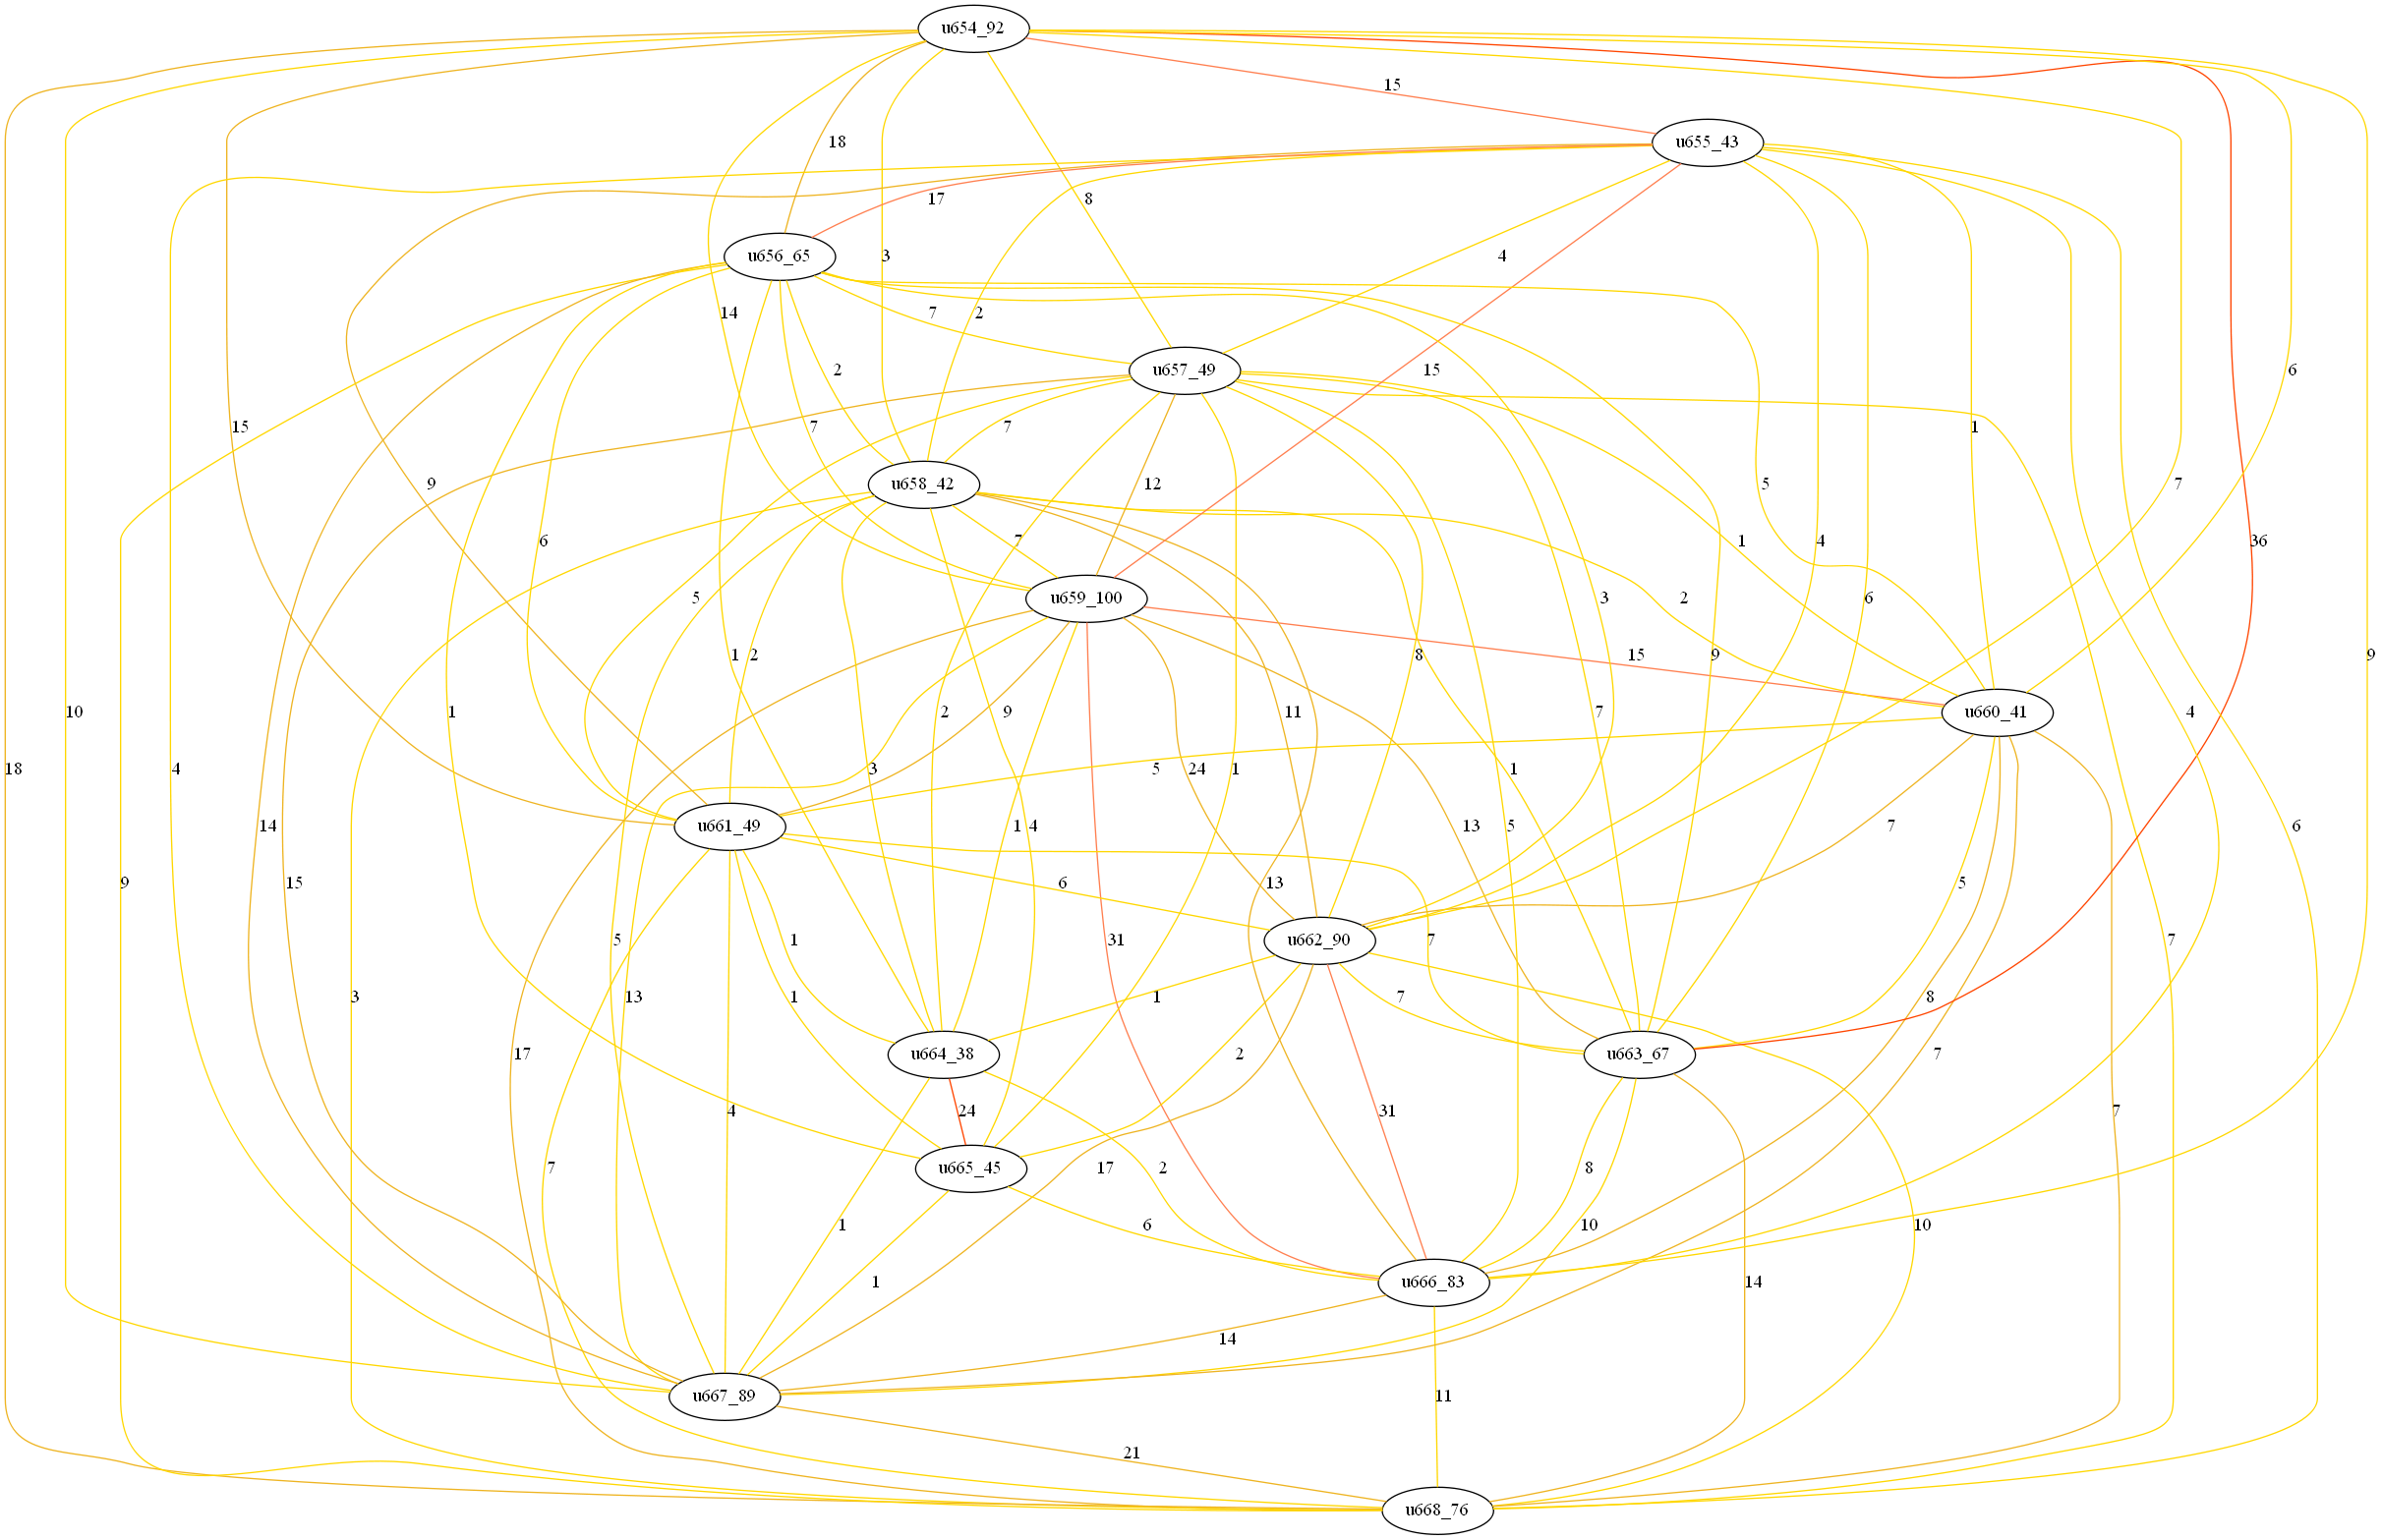
\includegraphics[scale=1.0]{"Computational Experiments/Inputs/inputEliteComPriorProfSemDispUn_201502011233270_/parUnidProfsComuns-EliteComPriorProfSemDispUn_201502011233270.png"}
\centering
\caption{Sharing of professors between blocks (school units) of scenario B1}
\end{figure}


%---------------
\item B2: Elite - com amarracao de disponib por unidade

\begin{figure}[H]
\includegraphics[scale=1.0]{"Computational Experiments/Inputs/inputEliteComPriorProfs_201501300027330_/parUnidProfsComuns-EliteComPriorProfs_201501300027330.png"}
\centering
\caption{Sharing of professors between blocks (school units) of scenario B2}
\end{figure}


%---------------
\item C: Elite ou Pensi - exemplo pequeno

%---------------
\item D: CEI

%---------------
\item E: Colegio Vicosa

\end{enumerate}


%%%%%%%%%%%%%%%%%%%%%%%%%%%%%%%%%%%%%%%%%%%%%%%%%%%%%%%%%%%%%%%%%%%%%%%%%%%%%%%%%%
\section{Approaches}

Different approaches and strategies for solving the problem were discussed at chapter ~\ref{chap:strategies}. Here some of these approaches are combined so that further various computational experiments are carried out and impacts of these distinct strategies are evaluated. The variations to be combined are briefly reviewed below.

\paragraph{Preemptive and Nonpreemptive Goal Programming}
The impact of ordered goals, their correlations, and trade-off situations are evaluated by solving the problem both with the preemptive goal programming and with an unified objective function.

\paragraph{Polishing method usage}
The need of the polishing method is demonstrated by optimizing the problem with and without it.

\paragraph{Professor Priority}
Professors priorities are evaluated using the three following perspectives:
\begin{enumerate}
\item No professor priority is considered: every goal of the problem is executed only once, considering all professors assignments without distinction.
\item Weak professor priority is considered: every goal of the problem is executed only once, but considering first-priority professors assignments more important than second-priority professors.
\item Strong professor priority is considered: every goal of the problem is executed twice. First, all goals are sequentially performed for all first-priority professors, then solution quality that was achieved for these professors is ensured and all goals are again sequentially performed for all second-priority professors.
\end{enumerate}

%Testes:
%
%23-02-15-NaraMaster-PensiSemNoitePriorProfs_201501291331550-priorTypeOff (Judas)
%21-02-15-NaraMaster-PensiSemNoitePriorProfs_201501291331550-priorTypeOffWeight (Slayer)
%21-02-15-NaraMaster-PensiSemNoitePriorProfs_201501291331550-priorType2 (Judas)
%
%23-02-15-NaraMaster-EliteComPriorProfSemDispUn_201502011233270-priorTypeOff (Slayer)
%22-02-15-NaraMaster-EliteComPriorProfSemDispUn_201502011233270-priorType2 (Slayer)
%24-02-15-NaraMaster-EliteComPriorProfSemDispUn_201502011233270-priorTypeOffWeight (PadreMarcelo)
%
%24-02-15-NaraMaster-EliteComPriorProfs_201501300027330-priorTypeOff (Slayer)
%26-02-14-NaraMaster-EliteComPriorProfs_201501300027330-priorType2 (PadreMarcelo rodando)
%26-02-14-NaraMaster-EliteComPriorProfs_201501300027330-priorTypeOffWeight (Slayer rodando)
%
%23-02-14-NaraMaster-PensiSemNoiteProfsImpo_201501291331550-priorTypeOffWeight (PadreMarcelo)

%%%%%%%%%%%%%%%%%%%%%%%%%%%%%%%%%%%%%%%%%%%%%%%%%%%%%%%%%%%%%%%%%%%%%%%%%%%%%%%%%%
\section{Results}

\subsection{Model features}

Following, model features for each instance are listed, which include the number of variables and restrictions created, detailed by type, and the reduced size of the model after applying Gurobi pre-solve method.


\subsection{Solver performance}

Whenever the solver is executed, analyzing performance and consequently the generated solution implies in analyzing every solving phase. This means checking for every step the running time, the optimization stopping condition that was reached, the best solution value of the linear program, the optimality gap and also how the solving process converged during the polishing method.


\subsection{Solution quality}

Evaluating quality of a final solution is not a trivial task, specially because there are multiple and conflicting goals involved. Often analyzing and understanding solutions require a deeper analysis of the problem data itself.

Following several solution quality indicators are listed and detailed for the experiments made.


